\documentclass[a4paper]{article}


%#########################################################################
\usepackage[utf8]{inputenc}
%\usepackage[T1]{fontenc}
%\usepackage[francais]{babel}
\usepackage[hmargin=4cm, vmargin=2cm, includeheadfoot]{geometry}
\usepackage{alltt}
\usepackage{multicol}
\usepackage{amsmath,amssymb}
\usepackage{color}
\usepackage{graphicx}
\usepackage[francais,bloc,completemulti]{automultiplechoice}     % Mandatory for conversion
\usepackage{mhchem} % needed for chemical equations
\usepackage{fp}
%\usepackage{tikz}

% Example of user macro
\providecommand{\abs}[1]{\lvert#1\rvert}
%#########################################################################
% Header
%#########################################################################

% Add test for graphic path [it works but fails if the compilation is performed from another folder]
% it could be fixer using TEXINPUTS
%\graphicspath{{Figures/other/}} 

\title{Test de conversion AMC vers moodle}
\author{amc2moodle team}



%#########################################################################
% Document
%#########################################################################
\begin{document}

% Define test level scoring
% e=incohérence; b=bonne; m=mauvaise; p planché (on ne descent pas en dessous)
\baremeDefautS{e=-0.5,b=1,m=-0.5}% never put b<1,
\baremeDefautM{e=-0.5,b=1,m=-0.25,p=-0.5}% never put b<1, with amc2moodle m correspond to the grade if all the wrong answers are ticked, b correspond to the grade if all the good answers are ticked

% Include tex file containing the questions
%amc2moodle \SetQuizOption{amc_aucune}{None of these answers are correct.}
%===================================================================
% simple
\element{cat1}{
  \begin{question}{Qsimple:img}
    On souhaite faire passer \textit{exactement}, par $N$ points donnés, un \texttt{polynôme} de degré \textbf{strictement} égal à $N-1$. Pour trouver les coefficients on doit résoudre un \emph{problème}
% Use "magic comments" to set imgResolution amc2moodle.
%amc2moodle \SetOption{imgResolution}{72}  
    \begin{center}
      \includegraphics[width=0.5\textwidth]{./Figures/other/schema_interpL.png}
    \end{center}

    \begin{reponses}
      \bonne{d'interpolation}
      \mauvaise{de moindre carré}
      \mauvaise{de Thelonius Sphere Monk
        \begin{flushright}
          \includegraphics[height=2cm]{./Figures/tinymonk.pdf}
        \end{flushright}
        \begin{flushleft}   
          \includegraphics[height=3cm]{./Figures/tinymonk.pdf}
        \end{flushleft}
      }
    \end{reponses}
  \end{question}
}


%===================================================================
% questions à réponse multiple
% pas de bonne réponse, on doit ajouter un champ "aucune de ces réponses n'est correcte"
% test for `\explain`.
% magic comment for feeback at question and answer level
\element{cat1}{
  \begin{questionmult}{Qmult:Aucune}  \bareme{e=-0.5,b=1,m=-1.,p=-0.5} % never put b<1,
    Quel fruit possède un noyau?
    \begin{reponseshoriz}[o] % keep answers order
      \mauvaise{La pomme}
      \mauvaise{La tomate}
      \mauvaise{
%amc2moodle \AddXMLAElement{feedback}{This is an \textbf{answer} feedback !}
      le Kiwi}
      %    \mauvaise{En allant à $$ \int_0^2 x \mathrm{d} x $$ la ligne}
    \end{reponseshoriz}
    \explain{Fruits grow on trees $x^3$, most of the \emph{time}.}
%amc2moodle \AddXMLQElement{partiallycorrectfeedback}{This is \textbf{partially} correct !}
%amc2moodle \SetOption{amc_aucune}{Aucune de ces réponses n'est correcte.}
  \end{questionmult}
}

%
% il y a des bonne réponses et un tableau, verbatim, macro
\element{cat2}{
  \begin{questionmult}{Qmult:TabVerbMacro}
    Quels sont les opérations qui donnent un chiffre présent dans le tableau?
    \begin{center}
      \begin{tabular}{ccc}
        \hline
        12                       & 2                                                    & $2^3$ \\
        \multicolumn{2}{c}{Deux} & \includegraphics[height=16pt]{4.png}         \\
        \hline
      \end{tabular}
    \end{center}
    \begin{reponses}
      \bonne{ Ou en \texttt{C} using \texttt{alltt} package
        \begin{alltt}
          int s=-2; \\
          for (int i=0;i<4; i++)\{ \\
          s=i*i+s; \\
          \}
        \end{alltt}
        %        \begin{verbatim}%L'environnement verbatim pose en effet des problèmes avec AMC
        %            int s=0
        %            for(int i;i=0; i<4){
        %                  s++
        %            }
        %        \end{verbatim}
      }
      \bonne{$\abs{-10-2}$ (math inline and newcommand)}
      \mauvaise{la réponse en image \includegraphics[height=16pt]{./Figures/other/4r.png}}
      \mauvaise{$6\times 6$}
      \mauvaise{Avec une équation  $$ \int_0^2 x \mathrm{d} x $$ } % works
      \bonne{Avec une équation matricielle
        \begin{equation}
          \mathrm{det} \begin{pmatrix}1 & 2 \\ -1 & 10 \end{pmatrix} = \begin{vmatrix}1 & 2 \\ -1 & 10 \end{vmatrix}
        \end{equation}
      }
      %    \mauvaise{Avec une autre équation utilisant \texttt{aligned} amsmath environnemnt
      %            \begin{equation}\left\{\begin{aligned}\displaystyle t_{0}&amp;\displaystyle=1/\sqrt{3}\\&#10;\displaystyle t_{i+1}&amp;\displaystyle=\frac{\sqrt{t_{i}^{2}+1}-1}{t_{i}}\end{aligned}\right..
      %            \end{equation}
      %    }
    \end{reponses}
  \end{questionmult}
}


% test with englisg keywords
% example from http://home.gna.org/auto-qcm/auto-multiple-choice.en/latex.shtml#latex.simple
\element{english}{
  \begin{question}{prez}
    Among the following persons, which one has ever been a President of the French Republic?
    \begin{choiceshoriz}
      \correctchoice{René Coty}
      \wrongchoice{Alain Prost}
      \wrongchoice{Marcel Proust}
      \wrongchoice{with an image \includegraphics[height=16pt]{./Figures/other/4r.png}}
    \end{choiceshoriz}
  \end{question}
}

% Test for local scoring
\element{english}{
  \begin{questionmult}{pref}     \scoring{e=-0.5,b=1,m=-.25,p=-0.5}
    Among the following cities, which ones are French prefectures?
    \begin{choices}
      \correctchoice{Poitiers}
      \wrongchoice{Sainte-Menehould}
      \correctchoice{Avignon}
    \end{choices}
  \end{questionmult}
}

% Test for itemize and enumerate and partial scoring
\element{cat1}{
\begin{question}{itemize-enumerate} \scoring{m=0,p=0}
Test for itemize html rendering,
\begin{itemize}
   \item first item
   \item Second item blablabla
\end{itemize}
test for enumerate html rendering,
\begin{enumerate}
  \item The first item $x^2$ with math
  \item The second \textbf{item } with bold
\end{enumerate}
    \begin{choices}
      \correctchoice{1 bullet list and 1 ordered list\\ Remarks: tags in item are ignored.}
      \wrongchoice{
        \begin{enumerate}
        \item The first item $x^2$
        \item The second \textbf{item}
        \end{enumerate}
    }
    \end{choices}
\end{question}
}


% Test for mhchem support with mathjax
\element{mhchem}{
\begin{question}{mathjax-mhchem}
Here is a test for \texttt{mhchem}-\LaTeX package. This package is not yet supported by LaTeXML, thus the rendering is delegated to \texttt{mathjax}. To use it, you need to add \texttt{mhchem} in the \texttt{mathjax} moodle plugin (ask to admin, see details in README file).


A complicated chemical equation \ce{Hg^2+ ->[I-] HgI2 ->[I-] [Hg^{II}I4]^2-}, the same written in math mode : $\ce{Hg^2+ ->[I-] HgI2 ->[I-] [Hg^{II}I4]^2-}$, combine with other math operator $K=\ce{Hg^2+ ->[I-] HgI2 ->[I-] [Hg^{II}I4]^2-}$ and finally placed in the equation environment
\begin{equation*}
K=\ce{Hg^2+ ->[I-] HgI2 ->[I-] [Hg^{II}I4]^2-}
\end{equation*}
% the answers
    \begin{choices}
      \correctchoice{a simpler one \ce{CO2 + C -> 2 CO}.}
      \wrongchoice{Wrong Choice! }
    \end{choices}
\end{question}
}

% Test for numerical question [other example in numerical.tex]
\element{num}{
\begin{questionmultx}{with-int}
Combien de fois le programme suivant affiche-t-il \texttt{"x"} ?

\texttt{for (int i = 4; i < 24; ++i)\\
\hspace*{1em}for (int j = i + 2; j - 1 > 0; -{}-j)\\
\hspace*{2em}puts("x");}

\AMCnumericChoices{290}{digits=3,sign=false,scoreexact=2,scoreapprox=1,approx=10}
\end{questionmultx}}


% Test for open question
\element{open}{
  \begin{question}{Essai}\label{q:Essai}   
    Explain in few words the aim of this course.
% It is possible to add more granularity with partially correct answer using \wrongchoice[P]{p}\scoring{0.5}
\AMCOpen{lines=2}{    \correctchoice[OK]{OK}    \wrongchoice[F]{F}}
  \end{question}
}

% Test for Description question
\element{desc}{
\begin{question}{pb-description} \QuestionIndicative
Provide a description of a problem that can be common to several questions. It is useful to define notation, pictures
\begin{center}
\includegraphics[height=32pt]{4.png}
\end{center}
equations $\int_0^1 x \mathrm{d} x = 0$\dots. Since, it is not a \emph{real} question, the \texttt{choices} environment is not provided. In this case, the question will be converted by \texttt{amc2moodle} into moodle \texttt{description} question type.

To use it in AMC, do not forget to use \texttt{QuestionIndicative} to tell AMC not to count points for this question (with a 0-point scoring).

% the associated scoring is \bareme{b=0,m=0,e=0,v=0} cf AMC doc
\end{question}
}

% Test for calculated question
\element{calc}{
\begin{question}{calc:area}\label{q:Calculated}
% Moodle requires at least one wild card in answer formula or question text
\FPseed=1 %  Defined but unused, because different random generator are used. 
\FPset{\x}{1}

\FPrandom{\y}

\FPeval{\a}{\x+random*(10-1)} % uniform in [1, 10]
\FPeval{\b}{1+\y*(10-1)} % uniform in [1, 10]
\FPeval{\c}{random * random} 

What is the \textbf{area} of rectangle of height \FPprint{\a} and width \FPprint{\b} ?

We recall that $\pi=$\FPpi .

Check for random labels : \FPprint{\c}

Check nested expression :
\FPeval{\nest}{ (1 + (pi+\x)/(pi-\x)) } \FPprint{\nest} =? 2.933884413848519720

Check for power and trigo :
% x^n -> pow(n, x)
$\sin(0.5)^2+\cos(0.5)^2$ = \FPeval{\trigo}{ pow(1+1, cos(0.5)) + pow(2, sin(0.5))} \FPprint{\trigo} =? 1


%Check FPseed : \the\FPseed

\begin{choices}
  \correctchoice{\FPprint{\FPeval{\out}{clip(\a *\b )}\out}}
  \wrongchoice{\FPprint{\FPeval{\out}{clip(\a +\b )}\out}}
\end{choices}
\end{question}
}

% -----------------------------------------------------------------------------
\element{calc}{
\begin{questionmult}{eig}\label{q:eig}  
% Define the random matrix parameter
\FPeval{\x}{1+random*(5-1)} % uniform in [1, 5]
\FPeval{\y}{1+random*(5-1)} % uniform in [1, 5]
\FPeval{\z}{1+random*(5-1)} % uniform in [1, 5]
Compute the eigenvalues of the following matrix
% moodle wilcards cannot be replaced inside equation 
\begin{equation}
\begin{pmatrix}
x & y \\
y & z
\end{pmatrix},
\end{equation}
where $x$=\FPprint{\x}, $y$=\FPprint{\y} and $z$=\FPprint{\z}.
% Define the characteristic polynomial coef
\FPeval{\a}{1}
\FPeval{\b}{neg(\x+\z)}
\FPeval{\c}{\x*\z-\y*\y}
% Résolution. Note \FPlsolve is not supported in amc2moodle
\FPeval{\disc}{(\b)*(\b) - 4*\a*\c}
\FPeval{\eigone}{(neg(\b) + root(2,\disc))/(2*\a)}
\FPeval{\eigtwo}{(neg(\b) - root(2,\disc))/(2*\a)}

% Use "magic comments" to set nitems and decimalNumber in amc2moodle
%amc2moodle \SetOption{nitems}{3}
%amc2moodle \SetOption{decimalNumber}{2}

\begin{choices}
  \correctchoice{\FPprint{\eigone}}
  \correctchoice{\FPprint{\eigtwo}}
  \wrongchoice{\FPprint{\disc}}
  \wrongchoice{\FPprint{\b}}
  \wrongchoice{\FPeval{\out}{\eigone+\eigtwo}\FPprint{\out}}
\end{choices}
\end{questionmult}
}
 % cat1, cat2, english, mhchem, num, open, desc
%% test for tikz 
\element{tikz}{
  \begin{question}{tikz:Q1}
    Among the following shape, where is the circle

    \begin{choices}
      \correctchoice{
\begin{tikzpicture}
          \draw (2,2) circle (1cm);
        \end{tikzpicture}}
      \wrongchoice{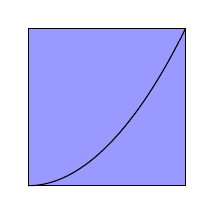
\begin{tikzpicture}
          \filldraw[fill=blue!40!white, draw=black] (0,0) rectangle (2,2);
          \draw (0,0) parabola (2,2);
        \end{tikzpicture}}
      \wrongchoice{$\triangle$}
    \end{choices}
  \end{question}
} % tikz


% #################################################################
% C R E A T I O N  D E S  C O P I E S
% #################################################################
\exemplaire{1}{    	% nombre de sujet différent
  %debut de l'en-tête des copies :    
  \vspace*{.5cm}
  \begin{minipage}{.4\linewidth}
    \centering\large\bf Test
  \end{minipage}
  \champnom{\fbox{
      \begin{minipage}{.5\linewidth}
        Nom et prénom :

        \vspace*{.5cm}\dotfill
        \vspace*{1mm}
      \end{minipage}
    }}

  \begin{flushleft}
Illustration of \texttt{amc2moodle} capabilities. All these questions can be converted \emph{automatically} to \texttt{moodle} with the same layout.
    \begin{center}
      \Large{\textsc{Multiple choice tests using AMC Latex Format}}\\
      \normalsize
    \end{center}
  \end{flushleft}


  % mélange et catégorie (groupe dans AMC)
  \cleargroup{BigGroupe}
  \copygroup{cat1}{BigGroupe}
  \copygroup{cat2}{BigGroupe}
  \copygroup{english}{BigGroupe}
  %\copygroup{tikz}{BigGroupe}
  \copygroup{mhchem}{BigGroupe}
  \copygroup{num}{BigGroupe}
  \copygroup{open}{BigGroupe}
  \copygroup{desc}{BigGroupe}
  \copygroup{calc}{BigGroupe}  
  % not usefull for testing !
  %\melangegroupe{BigGroupe}
  \restituegroupe{BigGroupe}
}


\end{document}
